% !TeX root = surprises.tex

\chapter{Wie man ein Museum bewacht}\label{c.museum}

%%%%%%%%%%%%%%%%%%%%%%%%%%%%%%%%%%%%%%%%%%%%%%%%%%%%%%%%%%%%%%%

1973 stellte Victor Klee die Frage, wie viele Wächter nötig sind, um alle Wände eines Museums zu überwachen. Wenn die Wände ein regelmäßiges Polygon oder sogar ein konvexes Polygon bilden, ist ein Wächter ausreichend (Abb.~\ref{f.museum.convex}).\index{Museum!guard a}

\begin{figure}[ht]
\begin{center}
\begin{tikzpicture}[scale=.6]
\coordinate (O) at (0,0);
\vertex{O};
\foreach \x/\name/\n/\po in {0/a/A/right,.6/b/B/above,1.6/c/C/left,2.4/d/D/below left,3.9/e/E/below right} {
  \coordinate (\name) at ($(O)+(\x*72+18:3cm)$);
\draw[dashed] (O) -- (\name);
}
\draw (a) -- (b) -- (c) -- (d) --(e) -- cycle;
\end{tikzpicture}
\end{center}
\caption{Ein Museum, dessen Wände ein konvexes Vieleck bilden}\label{f.museum.convex}
\end{figure}

Betrachten wir nun ein Museum mit sägezahnförmigen Wänden (Abb.~\ref{f.museum.nonconvex}). Überprüfen Sie durch Zählen, dass das Museum $15$ Wände hat. Jeder ``Zahn'' definiert ein Dreieck, das in Abb.~\ref{f.visibility-tooth} grau schattiert ist. Ein Wächter, der sich an einer beliebigen Stelle innerhalb eines der Dreiecke befindet, kann alle Wände beobachten, die dieses Dreieck begrenzen (rote Pfeile).
\begin{figure}[b]
\begin{center}
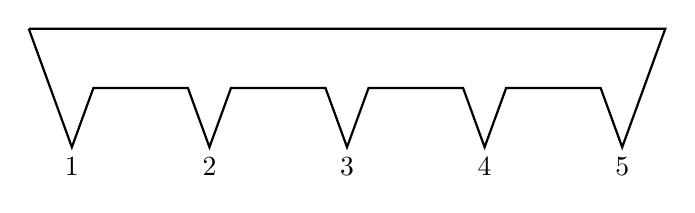
\begin{tikzpicture}[scale=.8]
\coordinate (O) at (0,0);
\draw [thick] (O) -- (++110:1cm) coordinate (P);
\draw[thick] (O) --
  ++(-70:1cm) coordinate(A) node[below] {$1$} -- 
  ++(+70:1cm) -- ++(0:1.5cm) --
  ++(-70:1cm) coordinate(B) node[below] {$2$} -- 
  ++(+70:1cm) -- ++(0:1.5cm) --
  ++(-70:1cm) coordinate(C) node[below] {$3$}-- 
  ++(+70:1cm) -- ++(0:1.5cm) --
  ++(-70:1cm) coordinate(D) node[below] {$4$} -- 
  ++(+70:1cm) -- ++(0:1.5cm) --
  ++(-70:1cm) coordinate(E) node[below] {$5$} --
  ++(+70:2cm) -- (P);
\end{tikzpicture}
\end{center}
\caption{Ein Museum, dessen Wände kein konvexes Vieleck bilden}\label{f.museum.nonconvex}
\end{figure}

\begin{figure}[t]
\begin{center}
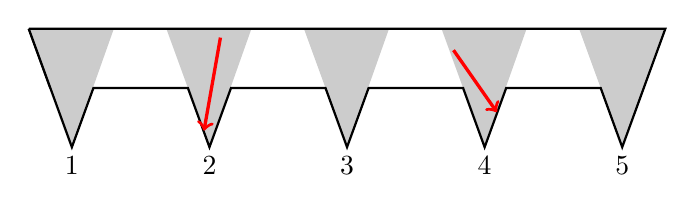
\begin{tikzpicture}[scale=.8]
\coordinate (O) at (0,0);
\draw [thick] (O) -- (++110:1cm) coordinate (P);
\path (O) --
  ++(-70:1cm) coordinate(A) node[below] {$1$} -- 
  ++(+70:1cm) coordinate(A1) -- ++(0:1.5cm) coordinate(A2) --
  ++(-70:1cm) coordinate(B) node[below] {$2$} -- 
  ++(+70:1cm) coordinate(B1) -- ++(0:1.5cm) coordinate(B2) --
  ++(-70:1cm) coordinate(C) node[below] {$3$}-- 
  ++(+70:1cm) coordinate(C1) -- ++(0:1.5cm) coordinate(C2) --
  ++(-70:1cm) coordinate(D) node[below] {$4$} -- 
  ++(+70:1cm) coordinate(D1) -- ++(0:1.5cm) coordinate(D2) --
  ++(-70:1cm) coordinate(E) node[below] {$5$} --
  ++(+70:2cm) coordinate(E1) -- (P);

\path[fill,black!20!white] (A) -- ++(110:2cm) -- ++(0:1.35cm)-- cycle;
\path[fill,black!20!white] (B) -- ++(110:2cm) -- ++(0:1.35cm)-- cycle;
\path[fill,black!20!white] (C) -- ++(110:2cm) -- ++(0:1.35cm)-- cycle;
\path[fill,black!20!white] (D) -- ++(110:2cm) -- ++(0:1.35cm)-- cycle;
\path[fill,black!20!white] (E) -- ++(110:2cm) -- ++(0:1.35cm)-- cycle;

\draw[thick] (P) -- (O) -- (A) -- (A1) -- (A2) --
   (B) -- (B1) -- (B2) -- (C) -- (C1) -- (C2) --
   (D) -- (D1) -- (D2) -- (E) -- (E1) -- (P);

\coordinate (G1) at (2.7,.8);
\coordinate (G2) at (6.4,.6);
\draw[->,red,very thick] (G1) -- +(-100:1.5cm);
\draw[->,red,very thick] (G2) -- +(-55:1.2cm);
\vertexcolor{G1}{red};
\vertexcolor{G2}{red};
\end{tikzpicture}
\end{center}
\caption{Sichtbarkeit innerhalb jedes ``Zahns''}\label{f.visibility-tooth}
\end{figure}

Wenn mindestens eine der Wachen in der Nähe der obersten Wand platziert ist, die das gesamte Museum überspannt, kann sie alle horizontalen Wände beobachten (blaue Pfeile in Abb.~\ref{f.museum.shaded}). Es genügen also $5=15/3$ Wächter, um alle Wände des Museums zu beobachten. Da sich die Dreiecke nicht überschneiden, kann eine Wache in einem Dreieck nicht alle Wände eines anderen Dreiecks beobachten (grüner Pfeil), so dass $5$ Wachen notwendig sind.

\begin{figure}[ht]
\begin{center}
\begin{tikzpicture}[scale=.8]
\coordinate (O) at (0,0);
\draw [thick] (O) -- (++110:1cm) coordinate (P);
\path (O) --
  ++(-70:1cm) coordinate(A) node[below] {$1$} -- 
  ++(+70:1cm) coordinate(A1) -- ++(0:1.5cm) coordinate(A2) --
  ++(-70:1cm) coordinate(B) node[below] {$2$} -- 
  ++(+70:1cm) coordinate(B1) -- ++(0:1.5cm) coordinate(B2) --
  ++(-70:1cm) coordinate(C) node[below] {$3$}-- 
  ++(+70:1cm) coordinate(C1) -- ++(0:1.5cm) coordinate(C2) --
  ++(-70:1cm) coordinate(D) node[below] {$4$} -- 
  ++(+70:1cm) coordinate(D1) -- ++(0:1.5cm) coordinate(D2) --
  ++(-70:1cm) coordinate(E) node[below] {$5$} --
  ++(+70:2cm) coordinate(E1) -- (P);

\path[fill,black!20!white] (A) -- ++(110:2cm) -- ++(0:1.35cm)-- cycle;
\path[fill,black!20!white] (B) -- ++(110:2cm) -- ++(0:1.35cm)-- cycle;
\path[fill,black!20!white] (C) -- ++(110:2cm) -- ++(0:1.35cm)-- cycle;
\path[fill,black!20!white] (D) -- ++(110:2cm) -- ++(0:1.35cm)-- cycle;
\path[fill,black!20!white] (E) -- ++(110:2cm) -- ++(0:1.35cm)-- cycle;

\draw[thick] (P) -- (O) -- (A) -- (A1) -- (A2) --
   (B) -- (B1) -- (B2) -- (C) -- (C1) -- (C2) --
   (D) -- (D1) -- (D2) -- (E) -- (E1) -- (P);

\coordinate (G1) at (9,.8);
\coordinate (G2) at ($(O)+(.5,.5)$);
\draw[->,very thick,green!80!black,dashed] (G1) -- +(-165:4.6cm);
\draw[->,very thick,blue] (G2) -- ++(7.4,.35);
\draw[->,very thick,blue] (G2) -- ++(2.9,-.42);
\draw[thick] (6,0) circle(4pt);
\draw[thick] (4.95,-.28) circle(4pt);
\vertexcolor{G1}{green!80!black};
\vertexcolor{G2}{blue};
\end{tikzpicture}
\end{center}
\caption{Sichtbarkeit der Wände des Museums}\label{f.museum.shaded}
\end{figure}

Das Beispiel in Abb.~\ref{f.museum.nonconvex} kann auf $n/3$ Zähne mit $n$ Wänden verallgemeinert werden, so dass wir schließen, dass \emph{mindestens} $n/3$ Wächter notwendig sind. Wir wollen beweisen, dass $n/3$ Wächter ausreichen, um ein beliebiges Museum zu bewachen.

Abschnitt~\ref{s.museum-triangulating} beweist, dass jedes triangulierte Polygon dreifarbig sein kann. Dies wird in Abschnitt~\ref{s.museum-guard} verwendet, um den Satz zu beweisen, dass $n/3$ Wächter ausreichend sind. Abschnitt~\ref{s.museum-trianguliert} vervollständigt den Beweis, indem er zeigt, dass jedes Polygon trianguliert werden kann.

\section{Dreieckige Polygone färben}\label{s.museum-triangulating}

\begin{definition}
Eine \emph{diagonal} a des Polygons ist eine Kante, die zwei Scheitelpunkte verbindet und nicht zu den (äußeren) Kanten des Polygons gehört.
\end{definition}

\begin{definition}
Ein Polygon ist dreieckig, wenn nicht schneidende Diagonalen so konstruiert werden können, dass das Innere des Polygons von Dreiecken bedeckt ist.
\end{definition}\index{Polygon!triangulated}

\begin{theorem}
Jedes beliebige Polygon kann trianguliert werden.\label{thm.tri}
\end{theorem}
Wir stellen den Beweis von Thm.~\ref{thm.tri} zurück.
\begin{definition}
Ein Eckpunkt eines Polygons ist \emph{konvex}\index{Polygon!konvexe und konkave Eckpunkte}, wenn sein Innenwinkel kleiner als $180^\circ$ ist; ein Eckpunkt ist \emph{konkav}, wenn sein Innenwinkel größer als $180^\circ$ ist. 
\end{definition}
In Abb.~\ref{f.museum.arbitrary} ist der Scheitelpunkt $1$ konvex und der Scheitelpunkt $2$ ist konkav.

\begin{figure}[ht]
\begin{center}
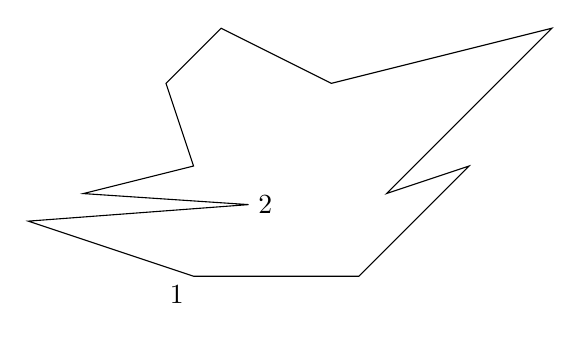
\begin{tikzpicture}[scale=.7]
\draw
  (0,0) coordinate (A) node[below left] {$1$} -- 
  ++(3,0) coordinate (B) --
  ++(2,2) coordinate (C) --
  ++(-1.5,-.5) coordinate (D) --
  ++(3,3) coordinate (E) -- 
  ++(-4,-1) coordinate (F) --
  ++(-2,1) coordinate (G) --
  ++(-1,-1) coordinate (H) --
  ++(.5,-1.5) coordinate (I) --
  ++(-2,-.5) coordinate (J) --
  ++(3,-.2) coordinate (K) node[right] {$2$} -- 
  ++(-4,-.3) coordinate (L) --
  cycle;
\vertex{A};
\vertex{K};
\end{tikzpicture}
\end{center}
\caption{Ein Polygon mit einem konvexen Scheitelpunkt ($1$) und einem konkaven Scheitelpunkt ($2$)}\label{f.museum.arbitrary}
\end{figure}

\begin{definition}
Ein Polygon mit Scheitelpunkten $V$ kann \emph{dreifarbig} sein, wenn es eine Karte gibt:
\[
c: V \mapsto \{\mathit{red},\mathit{blue},\mathit{green}\}\,,
\]
so dass keine Kante zwei Scheitelpunkte hat, denen die gleiche Farbe zugewiesen ist.
\end{definition}

\begin{theorem}
Ein dreieckiges Polygon kann dreifarbig sein.\label{thm.colored}
\end{theorem}\index{Coloring!polygon@of a polygon}

\begin{proof}
Durch Induktion auf die Anzahl der Scheitelpunkte. Ein Dreieck kann dreifarbig sein. Ein dreieckiges Polygon mit $n>3$ Scheitelpunkten muss eine Diagonale haben. Wähle eine beliebige Diagonale $\overline{AB}$ (Abb.~\ref{f.museum.three-1}) und teile das Polygon entlang dieser Diagonale in zwei kleinere Polygone (Abb.~\ref{f.museum.three-2}). Durch Induktion kann jedes dieser kleineren Polygone dreifarbig sein (Abb.~\ref{f.museum.three-3}).

Da die zugewiesenen Farben willkürlich sind, können wir, wenn $A,B$ in den beiden Polygonen unterschiedliche Farben zugewiesen werden, die Farben in einem der beiden Polygone umbenennen, so dass die Farben von $A,B$ in beiden Polygonen gleich sind. In Abb.~\ref{f.museum.three-4} tauschen Sie zum Beispiel \emph{rot} und \emph{grün} im unteren Polygon aus.
Fügen Sie die beiden Polygone zusammen, um das ursprüngliche Polygon mit $n$ Scheitelpunkten zu erhalten. Es wird dreifarbig sein (Abb.~\ref{f.museum.three-5}).
\end{proof}

\begin{figure}[t]
\begin{minipage}{.45\textwidth}
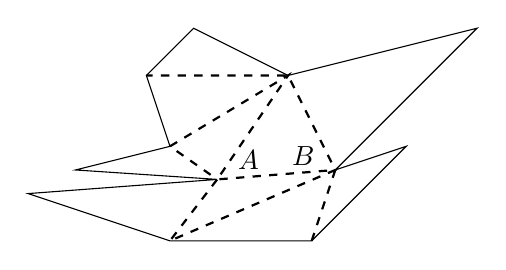
\begin{tikzpicture}[scale=.6]
\draw
  (0,0) coordinate (A) -- 
  ++(3,0) coordinate (B) --
  ++(2,2) coordinate (C) --
  ++(-1.5,-.5) coordinate (D) --
  ++(3,3) coordinate (E) -- 
  ++(-4,-1) coordinate (F) --
  ++(-2,1) coordinate (G) --
  ++(-1,-1) coordinate (H) --
  ++(.5,-1.5) coordinate (I) --
  ++(-2,-.5) coordinate (J) --
  ++(3,-.2) coordinate (K) -- 
  ++(-4,-.3) coordinate (L) --
  cycle;
\vertex{K};
\vertex{D};
\node[above right,xshift=4pt] at (K) {$A$};
\node[above left,xshift=-4pt,yshift=-2pt] at (D) {$B$};

\draw[thick,dashed]
  (B) -- (D) -- (K) -- (F) -- (I) -- (K) -- (A) -- (D) -- (F) -- (H);
\end{tikzpicture}
\caption{Eine beliebige Diagonale in einem Polygon}\label{f.museum.three-1}
\end{minipage}
\hfill
\begin{minipage}{.45\textwidth}
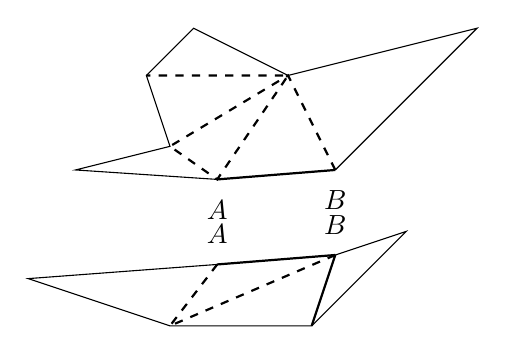
\begin{tikzpicture}[scale=.6]
\path
  (0,0) coordinate (A1) -- 
  ++(3,0) coordinate (B1) --
  ++(2,2) coordinate (C1) --
  ++(-1.5,-.5) coordinate (D1);
\draw
  (D1) --
  ++(3,3) coordinate (E1) -- 
  ++(-4,-1) coordinate (F1) --
  ++(-2,1) coordinate (G1) --
  ++(-1,-1) coordinate (H1) --
  ++(.5,-1.5) coordinate (I1) --
  ++(-2,-.5) coordinate (J1) --
  ++(3,-.2) coordinate (K1);
\path
  (K1) -- 
  ++(-4,-.3) coordinate (L1) --
  (A1);
\vertex{K1};
\vertex{D1};
\node[below,yshift=-4pt] at (K1) {$A$};
\node[below,yshift=-4pt] at (D1) {$B$};

\draw[thick,dashed]
  (D1) -- (F1) -- (I1) -- (K1) -- (F1) -- (H1);
\draw[thick] (D1) -- (K1);

\begin{scope}[yshift=-1.8cm]
\draw
  (0,0) coordinate (A2) -- 
  ++(3,0) coordinate (B2) --
  ++(2,2) coordinate (C2) --
  ++(-1.5,-.5) coordinate (D2);
\path
  (D2) --
  ++(3,3) coordinate (E2) --
  ++(-4,-1) coordinate (F2) --
  ++(-2,1) coordinate (G2) --
  ++(-1,-1) coordinate (H2) --
  ++(.5,-1.5) coordinate (I2) --
  ++(-2,-.5) coordinate (J2) --
  ++(3,-.2) coordinate (K2);
\draw
  (K2) --
  ++(-4,-.3) coordinate (L2) --
  (A2);
\vertex{K2};
\vertex{D2}; 
\node[above,yshift=4pt] at (K2) {$A$};
\node[above,yshift=4pt] at (D2) {$B$};

\draw[thick,dashed]
  (K2) -- (A2) -- (D2) -- (B2) -- (D2);
\draw[thick] (D2) -- (K2);
\end{scope}
\end{tikzpicture}
\caption{Teilen Sie das Polygon}\label{f.museum.three-2}
\end{minipage}
\end{figure}

\begin{figure}[t]
\begin{minipage}{.45\textwidth}
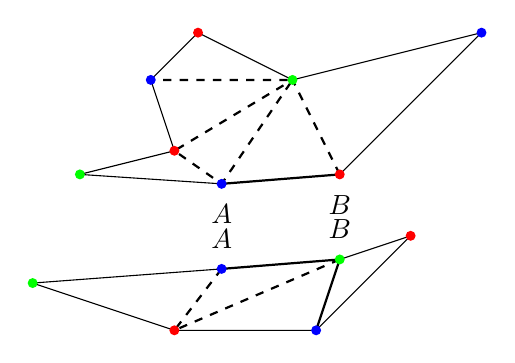
\begin{tikzpicture}[scale=.6]
\path
  (0,0) coordinate (A1) -- 
  ++(3,0) coordinate (B1) --
  ++(2,2) coordinate (C1) --
  ++(-1.5,-.5) coordinate (D1);
\draw
  (D1) --
  ++(3,3) coordinate (E1) -- 
  ++(-4,-1) coordinate (F1) --
  ++(-2,1) coordinate (G1) --
  ++(-1,-1) coordinate (H1) --
  ++(.5,-1.5) coordinate (I1) --
  ++(-2,-.5) coordinate (J1) --
  ++(3,-.2) coordinate (K1);
\path
  (K1) -- 
  ++(-4,-.3) coordinate (L1) --
  (A1);
  
\draw[thick,dashed]
  (D1) -- (F1) -- (I1) -- (K1) -- (F1) -- (H1);
\draw[thick] (D1) -- (K1);

\node[below,yshift=-4pt] at (K1) {$A$};
\node[below,yshift=-4pt] at (D1) {$B$};

\foreach \point/\color in {D1/red,E1/blue,F1/green,G1/red,H1/blue,I1/red,J1/green,K1/blue}
  \fill[color=\color] (\point) circle(3pt);

\begin{scope}[yshift=-1.8cm]

\draw
  (0,0) coordinate (A2) -- 
  ++(3,0) coordinate (B2) --
  ++(2,2) coordinate (C2) --
  ++(-1.5,-.5) coordinate (D2);
\path
  (D2) --
  ++(3,3) coordinate (E2) --
  ++(-4,-1) coordinate (F2) --
  ++(-2,1) coordinate (G2) --
  ++(-1,-1) coordinate (H2) --
  ++(.5,-1.5) coordinate (I2) --
  ++(-2,-.5) coordinate (J2) --
  ++(3,-.2) coordinate (K2);
\draw
  (K2) --
  ++(-4,-.3) coordinate (L2) --
  (A2);
  
\draw[thick,dashed]
  (K2) -- (A2) -- (D2) -- (B2) -- (D2);
\draw[thick] (D2) -- (K2);
\node[above,yshift=4pt] at (K2) {$A$};
\node[above,yshift=4pt] at (D2) {$B$};

\foreach \point/\color in {A2/red,B2/blue,C2/red,D2/green,K2/blue,L2/green}
  \fill[color=\color] (\point) circle(3pt);

\end{scope}
\end{tikzpicture}
\caption{Dreifarbige Darstellung der beiden kleineren Polygone}\label{f.museum.three-3}
\end{minipage}
\hfill
\begin{minipage}{.45\textwidth}
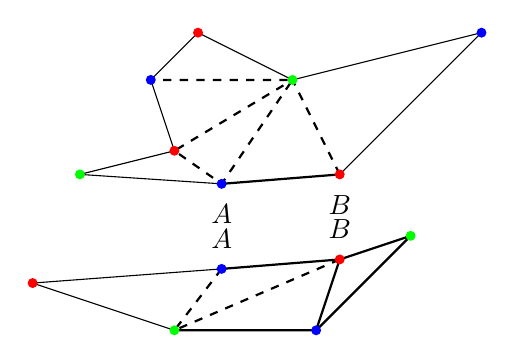
\begin{tikzpicture}[scale=.6]
\path
  (0,0) coordinate (A1) -- 
  ++(3,0) coordinate (B1) --
  ++(2,2) coordinate (C1) --
  ++(-1.5,-.5) coordinate (D1);
\draw
  (D1) --
  ++(3,3) coordinate (E1) -- 
  ++(-4,-1) coordinate (F1) --
  ++(-2,1) coordinate (G1) --
  ++(-1,-1) coordinate (H1) --
  ++(.5,-1.5) coordinate (I1) --
  ++(-2,-.5) coordinate (J1) --
  ++(3,-.2) coordinate (K1);
\path
  (K1) -- 
  ++(-4,-.3) coordinate (L1) --
  (A1);
  
\node[below,yshift=-4pt] at (K1) {$A$};
\node[below,yshift=-4pt] at (D1) {$B$};

\draw[thick,dashed]
  (D1) -- (F1) -- (I1) -- (K1) -- (F1) -- (H1);
\draw[thick] (D1) -- (K1);

\foreach \point/\color in {D1/red,E1/blue,F1/green,G1/red,H1/blue,I1/red,J1/green,K1/blue}
  \fill[color=\color] (\point) circle(3pt);

\begin{scope}[yshift=-1.8cm]

\draw[thick]
  (0,0) coordinate (A2) -- 
  ++(3,0) coordinate (B2) --
  ++(2,2) coordinate (C2) --
  ++(-1.5,-.5) coordinate (D2);
\path
  (D2) --
  ++(3,3) coordinate (E2) --
  ++(-4,-1) coordinate (F2) --
  ++(-2,1) coordinate (G2) --
  ++(-1,-1) coordinate (H2) --
  ++(.5,-1.5) coordinate (I2) --
  ++(-2,-.5) coordinate (J2) --
  ++(3,-.2) coordinate (K2);
\draw
  (K2) --
  ++(-4,-.3) coordinate (L2) --
  (A2);
  
\draw[thick,dashed]
  (K2) -- (A2) -- (D2) -- (B2) -- (D2);
\draw[thick] (D2) -- (K2);
\node[above,yshift=4pt] at (K2) {$A$};
\node[above,yshift=4pt] at (D2) {$B$};

\foreach \point/\color in {A2/green,B2/blue,C2/green,D2/red,K2/blue,L2/red}
  \fill[color=\color] (\point) circle(3pt);

\end{scope}
\end{tikzpicture}
\caption{Tauschen Sie die Farben eines Polygons aus, um sie an das andere anzupassen.}\label{f.museum.three-4}
\end{minipage}
\end{figure}

\begin{figure}[t]
\begin{center}
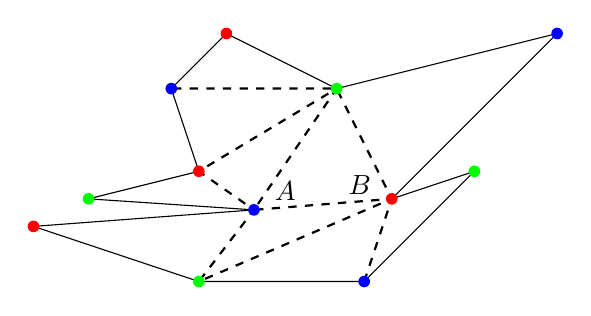
\begin{tikzpicture}[scale=.7]
\draw
  (0,0) coordinate (A) -- 
  ++(3,0) coordinate (B) --
  ++(2,2) coordinate (C) --
  ++(-1.5,-.5) coordinate (D) --
  ++(3,3) coordinate (E) -- 
  ++(-4,-1) coordinate (F) --
  ++(-2,1) coordinate (G) --
  ++(-1,-1) coordinate (H) --
  ++(.5,-1.5) coordinate (I) --
  ++(-2,-.5) coordinate (J) --
  ++(3,-.2) coordinate (K) -- 
  ++(-4,-.3) coordinate (L) --
  cycle;
  
\node[above right,xshift=4pt] at (K) {$A$};
\node[above left,xshift=-4pt,yshift=-2pt] at (D) {$B$};

\draw[thick,dashed]
  (B) -- (D) -- (K) -- (F) -- (I) -- (K) -- (A) -- (D) -- (F) -- (H);

\foreach \point/\color in {D/red,E/blue,F/green,G/red,H/blue,I/red,J/green,K/blue,A/green,B/blue,C/green,L/red}
  \fill[color=\color] (\point) circle(3pt);

\end{tikzpicture}
\end{center}
\caption{Fügen Sie die beiden kleineren Polygone wieder zusammen}\label{f.museum.three-5}
\end{figure}

\section{Vom Färben von Polygonen zum Bewachen eines Museums}\label{s.museum-guard}

\begin{theorem}\label{thm.guarded} Ein Museum mit $n$ Wänden kann von $n/3$ Wächtern bewacht werden.
\end{theorem}\index{Museum!triangulated@and triangulated polygons}
\begin{proof}
Durch Thm.~\ref{thm.tri} kann das Polygon trianguliert werden und durch Thm.~\ref{thm.colored} kann das Polygon dreifarbig sein. Alle drei Eckpunkte jedes Dreiecks in der Triangulation müssen mit \emph{unterschiedlichen} Farben gefärbt sein, um die Bedingung der Dreifarbigkeit zu erfüllen. Da das Polygon dreifarbig ist, kann mindestens eine Farbe, z.B. Rot, höchstens $n/3$ mal vorkommen, und jedes Dreieck muss einen rot gefärbten Scheitelpunkt haben. Stationiere eine Wache an jedem roten Scheitelpunkt; sie kann alle Wände des Dreiecks beobachten, zu dem der Scheitelpunkt gehört. Da die Dreiecke der Triangulation alle Kanten des Polygons umfassen, reichen $n/3$ Wächter aus, um alle Wände des Museums zu beobachten.
\end{proof}
Wenn $n$ nicht durch $3$ teilbar ist, ist die Anzahl der benötigten Wächter $\lfloor n/3\rfloor$, die größte ganze Zahl kleiner oder gleich $n/3$. Für Museen mit $12, 13, 14$ Wänden reichen beispielsweise $4$ Wachen aus, da $\lfloor 12/3\rfloor =\lfloor 13/3\rfloor=\lfloor 14/3\rfloor=4$. Der Einfachheit halber ignorieren wir diese Komplikation.
 
\subsection{Beliebige Polygone können trianguliert werden}\label{s.museum-trianguliert}

\begin{theorem}\label{thm.interior-angles-of-a-polygon}
Die Summe der Innenwinkel eines Polygons mit $n$ Scheitelpunkten ist:
\[180^\circ(n-2)\,.\]
\end{theorem}\index{Polygon!trianguliert}
\begin{proof}
Man betrachte ein konvexes Polygon und bezeichne seine \emph{Außenwinkel} mit $\theta_i$ (Abb.~\ref{f.museum.exterior}).
Wenn man sich von einer gestrichelten Linie zur nächsten bewegt, vollzieht man eine Drehung um einen Kreis, so:
\[
\sum_{i=1}^n \theta_i = 360^\circ\,.
\]
\begin{figure}[t]
\begin{center}
\begin{tikzpicture}[scale=.5]
\coordinate (O) at (0,0);
\foreach \x/\name/\n/\po in {0/a/A/right,.6/b/B/above,1.6/c/C/left,2.4/d/D/below left,3.9/e/E/below right} {
  \coordinate (\name) at ($(O)+(\x*72+18:3cm)$);
}
\draw[thick] (a) -- (b) -- (c) -- (d) --(e) -- cycle;

\draw[thick,dashed] (a) 
  node[above,xshift=-2pt,yshift=8pt] {$\theta_1$} -- 
  ($(a)!2!(b)$);
\draw[thick,dashed] (b)
  node[above left,xshift=-8pt,yshift=0pt] {$\theta_2$} -- 
  ($(b)!1.7!(c)$);
\draw[thick,dashed] (c) 
  node[below left,xshift=-4pt,yshift=-2pt] {$\theta_3$} -- 
  ($(c)!1.7!(d)$);
\draw[thick,dashed] (d)
  node[below right,xshift=0pt,yshift=-4pt] {$\theta_4$} -- 
  ($(d)!1.5!(e)$);
\draw[thick,dashed] (e)
  node[right,xshift=4pt,yshift=4pt] {$\theta_5$} -- 
  ($(e)!1.7!(a)$);

\end{tikzpicture}
\end{center}
\caption{Die Außenwinkel eines konvexen Polygons}\label{f.museum.exterior}
\end{figure}
Für jeden Außenwinkel $\theta_i$ bezeichne man den entsprechenden Innenwinkel mit $\phi_i$. Dann:
\begin{eqnarray*}
\displaystyle\sum_{i=1}^n \theta_i &=&\displaystyle\sum_{i=1}^n (180^\circ-\phi_i)= 360^\circ\\
\displaystyle\sum_{i=1}^n \phi_i &=& n\cdot 180^\circ-360^\circ =180^\circ(n-2)\,.
\end{eqnarray*}
Wenn es einen konkaven Scheitelpunkt gibt ($B$ in Abb.~\ref{f.museum.concave}), gibt es ein Dreieck, das von den beiden Kanten, die auf den konkaven Scheitelpunkt treffen, und der Linie $\overline{AC}$, die die beiden anderen Scheitelpunkte verbindet, gebildet wird. Summiert man die Winkel des Dreiecks, so erhält man:
\begin{eqnarray*}
(180^\circ - \alpha) + (360^\circ - \beta) + (180^\circ - \gamma) &=& 180^\circ\\
\alpha + \beta + \gamma &=& 3\cdot 180^\circ\,.
\end{eqnarray*}

Die Summe der Innenwinkel nimmt um $\alpha+\beta+\gamma$ zu, während die Anzahl der Scheitelpunkte um drei zunimmt, so dass die Gleichung im Theorem erhalten bleibt:
\begin{eqnarray*}
\displaystyle\sum_{i=1}^n \phi_i + (\alpha + \beta + \gamma) &=& 180^\circ(n-2)+3\cdot 180^\circ\\
&=& 180^\circ((n+3)-2)\,.
\end{eqnarray*}
\end{proof}

\begin{figure}[t]
\begin{center}
\begin{tikzpicture}[scale=.8]
\draw[thick] (0,0) -- 
  (3,0) coordinate (A) node[above left,yshift=8pt] {$\alpha$} --
  ++(60:2) coordinate (B) node[above,yshift=8pt] {$\beta$} --
  ++(-60:2) coordinate (C) 
    node[above right,yshift=8pt] {$\gamma$}  --
  ++(3,0);

\draw ($(A)+(-.4,0)$) arc(180:60:.4);
\draw ($(B)+(-60:.3)$) arc(-60:240:.3);
\draw ($(C)+(.4,0)$) arc(0:120:.4);
\node[below] at (A) {$A$};
\node[below,yshift=-5pt] at (B) {$B$};
\node[below] at (C) {$C$};
\draw[thick,dashed] (A) -- (C);
\end{tikzpicture}
\end{center}
\caption{Ein konkaver Scheitelpunkt}\label{f.museum.concave}
\end{figure}


\begin{theorem}\label{thm.convex}
Ein Polygon muss mindestens drei konvexe Scheitelpunkte haben.
\end{theorem}

\begin{proof}
Sei $k$ die Anzahl der konkaven Scheitelpunkte, deren Innenwinkel $180^\circ+\epsilon_i$ ist, $\epsilon_i>0$. Die Summe der Innenwinkel der \emph{konkaven} Scheitelpunkte ist sicher kleiner oder gleich der Summe der Innenwinkel von \emph{allen} Scheitelpunkten:
\begin{eqnarray*}
k\cdot 180^\circ +\displaystyle\sum_{i=1}^{k}\epsilon_i &\leq& 180^\circ(n-2)\\
(k+2)\cdot 180^\circ +\displaystyle\sum_{i=1}^{k}\epsilon_i &\leq& n\cdot 180^\circ\\
(k+2)\cdot 180^\circ &<& n\cdot 180^\circ\\
k&<&n-2\,.
\end{eqnarray*}
Daraus folgt, dass es mindestens drei Scheitelpunkte geben muss, die konvex und nicht konkav sind.
\end{proof}

\begin{proof}[Theorem~\ref{thm.tri}]
Durch Induktion auf die Anzahl der Scheitelpunkte. Für $n=3$ gibt es nichts zu beweisen. Wenn $n>3$, muss es nach Thm.~\ref{thm.convex} einen konvexen Scheitelpunkt $C$ geben. Beschrifte seine benachbarten Scheitelpunkte mit $B,D$. Wenn $\overline{BD}$ im Polygon enthalten ist (Abb.~\ref{f.contained}), ist sie eine Diagonale und das Polygon kann in ein $\triangle BCD$ und ein weiteres Polygon $\overline{ABDE}$ mit $\overline{BD}$ als Kante zerlegt werden, das kleiner als das ursprüngliche Polygon ist (Abb.~\ref{f.contained}). Durch die induktive Hypothese kann das Polygon trianguliert und dann wieder in das $\triangle BCD$ eingefügt werden, wodurch das ursprüngliche Polygon trianguliert wird.

\begin{figure}[t]
\begin{minipage}{.45\textwidth}
\begin{tikzpicture}[scale=1.4]
\clip (-.5,-.4) rectangle (3.8,2.2);
\draw
  (0,0) coordinate (A) -- 
  ++(1.5,0) coordinate (B) --
  ++(2,2) coordinate (C) --
  ++(-1.8,-.5) coordinate (D) --
  ++(-1,.5) coordinate (E) --
  (A);
\draw[thick,dashed] (B) -- (D);
\foreach \point/\pos in {A/below,B/below,C/right,D/above,E/left}
  \node[\pos] at (\point) {$\point$};
\vertex{B};
\vertex{D};
\end{tikzpicture}
\caption{Triangulation, bei der eine Diagonale im Polygon enthalten ist}\label{f.contained}
\end{minipage}
\hfill
\begin{minipage}{.45\textwidth}
\begin{tikzpicture}[scale=1.4]
\clip (-.2,-.4) rectangle (3.8,2.2);
\draw
  (0,0) coordinate (A) -- 
  ++(1.5,0) coordinate (B) --
  ++(2,2) coordinate (C) --
  ++(-1.8,-.5) coordinate (D) --
  ++(-1,.5) coordinate (E) --
  ++(1.3,-1) coordinate (F) --
  (A);
\draw[thick,dashed] (B) -- (D);
\draw[very thick,dotted] (C) -- (F);
\node [draw,circle through=(F)] at (C) {};
\node[below] at (A) {$A$};
\node[below] at (B) {$B$};
\node[right] at (C) {$C$};
\node[above,yshift=2pt,xshift=-3pt] at (D) {$D$};
\node[left]  at (E) {$E$};
\node[below,yshift=-1pt,xshift=-2pt] at (F) {$F$};
\vertex{C};
\vertex{F};
\end{tikzpicture}
\caption{Triangulation, bei der eine Diagonale nicht im Polygon enthalten ist}\label{f.museum.concave-vertices}
\end{minipage}
\end{figure}
Wenn $\overline{BD}$ nicht im Polygon enthalten ist, muss es einen konkaven Scheitelpunkt $F$ geben, der $C$ am nächsten liegt (Abb.~\ref{f.museum.concave-vertices}). $\overline{CF}$ ist eine Diagonale und zerlegt das Polygon in zwei kleinere Polygone $\overline{CFED}$ und $\overline{CFAB}$. Durch die Induktionshypothese können diese trianguliert und zusammengeklebt werden.
\end{proof}

\subsection*{Was ist die Überraschung?}
Das Museumstheorem ist überraschend, denn was wie ein Theorem in der Geometrie aussieht, wird recht elegant durch einen Appell zur Färbung eines Graphen bewiesen.

\subsection*{Quellen}

Dieses Kapitel basiert auf \cite[Chap.~39]{thebook}.
